% Template for ICIP-2019 paper; to be used with:
%          spconf.sty  - ICASSP/ICIP LaTeX style file, and
%          IEEEbib.bst - IEEE bibliography style file.
% --------------------------------------------------------------------------
\documentclass{article}
\usepackage{spconf,amsmath,graphicx}

% Example definitions.
% --------------------
\def\x{{\mathbf x}}
\def\L{{\cal L}}

% Title.
% ------
\title{AUTHOR GUIDELINES FOR ICIP 2019 PROCEEDINGS MANUSCRIPTS}
%
% Single address.
% ---------------
\name{Author(s) Name(s)\thanks{Thanks to XYZ agency for funding.}}
\address{Author Affiliation(s)}
%
% For example:
% ------------
%\address{School\\
%	Department\\
%	Address}
%
% Two addresses (uncomment and modify for two-address case).
% ----------------------------------------------------------
%\twoauthors
%  {A. Author-one, B. Author-two\sthanks{Thanks to XYZ agency for funding.}}
%	{School A-B\\
%	Department A-B\\
%	Address A-B}
%  {C. Author-three, D. Author-four\sthanks{The fourth author performed the work
%	while at ...}}
%	{School C-D\\
%	Department C-D\\
%	Address C-D}
%
\begin{document}
%\ninept
%
\maketitle
%
\begin{abstract}
The abstract should appear at the top of the left-hand column of text, about
0.5 inch (12 mm) below the title area and no more than 3.125 inches (80 mm) in
length.  Leave a 0.5 inch (12 mm) space between the end of the abstract and the
beginning of the main text.  The abstract should contain about 100 to 150
words, and should be identical to the abstract text submitted electronically
along with the paper cover sheet.  All manuscripts must be in English, printed
in black ink.
\end{abstract}
%
\begin{keywords}
One, two, three, four, five
\end{keywords}
%
\section{Introduction}
\label{sec:intro}

Despite its apparent success in a variety of tasks from robotics to game playing, Deep Reinforcement Learning raises a number of issues on the matter of generalization. The attractiveness of this paradigm is owed in no small part to its general aspect; ideally, the same model would be able to learn any task as long as the environment it is put in is correctly and optimally designed. Consequently, Deep Reinforcement Learning techniques attract interest for their great potential for transfer across applications with little to no adjustments. Efforts towards reaching this goal are however impeded in a number of ways. 
Deep reinforcement learning models often suffer of high sample complexity. Policy gradients estimates have high variance and have shown  to be extremely sensitive to hyperparameter choices, network architecture, environment-specific variables, as well as random seeds. [cite: drl that matters?] %They also have a tendency to overfit to their training environment.
 This not only makes reproducing the reported results of a given technique a hard and unpredictable task, it also seemingly cancels the advantage of having a general paradigm for transfer across applications as it creates a need for fine-tuning the model for any given non-trivial task.

Policy Gradient methods are particularly attractive because they are straightforward to combine with nonlinear approximators such as neural networks. Those estimators however suffer from extremely high variance, and necessitate a very large number of samples. Actor critic method try to solve this by introducing value functions, which sensibly reduces variance and the size of needed samples, at the cost of creating bias. There are several kinds of value functions and different methods to estimate them, and the aim is to find an estimator that reduces optimally the variance without creating a poor solution from too much bias.

Motivation for our method:
- facilitate finding the balance/an optimal estimate in terms of variance and bias --> reduce the need to fine-tune the model and generalize better.

(Research about: the relationship between Ensemble Learning, Advantage Estimation, and the variance and bias trade-off)

(Also: Ensemble Learning and the different advantage estimation techniques)

In this paper, we investigate the effects of using network ensemble for advantage estimation. The goal of this experiment is to see how this method affects the performance of advantage-based actor-critic methods. The intuition behind this method is that it could help training multiple advantage estimation methods with different hyperparameters would require less fine-tuning to specific environments and algorithms, leading to better generalization. 


The experiment plan includes:  
- training multiple estimation methods with different hyperparameters.
- testing different rules for combining the estimates obtained from each network.
- testing different advantage-based actor-critic algorithms and noting the impact on their performance. 

- to find an estimation that introduces minimal bias while reducing the variance, and 

- Ensemble network
- Advantage based actor critic method
- critic = advantage estimation. Trained with supervised learning? mean squared error
- advantage estimation by multiple neural networks
- network ensemble 


\section{Preliminaries}
\label{sec:format}

For a policy $\pi$ with parameters $\theta$ we give the following policy gradient formula below:
%\[
%g = \mathbb{E}[\sum_{t=0}{\infty} \Psi \nabla_{\theta}\log\pi_{\theta}(a_t|s_t)]
%\]

The weight $\Psi$ has a number of different possible values, like the total reward, the TD residual, the state-value function or the advantage function. The advantage function $A^\pi(s_t, a_t)$ is the most optimal choice for lowering variance. We estimate this function by a neural network called the Critic network.

\section{PAGE TITLE SECTION}
\label{sec:pagestyle}

%Test the method with different algorithms
%they need to be actor-critic algorithms
%will our method be implemented differently to include each algorithm's tricks? or will we only implement it on top of algorithms that do not require modifications?

%tableaux : lignes: algorithmes2baz, algorithmes + amélioration, algorithmes + améliorations d'autres articles. colonnes : tasks

%\begin{tabular}
%\end{tabular}

\begin{figure}[htb]
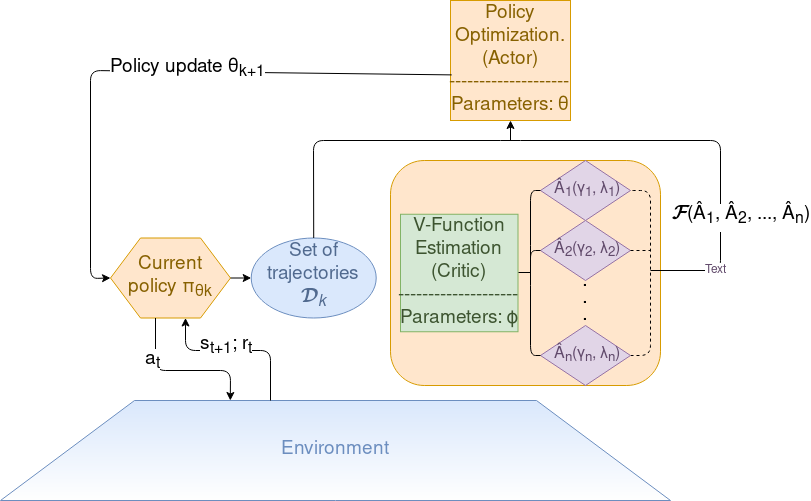
\includegraphics[width=8.5cm]{model}
\caption{Multi-advantage critic}
\label{fig:model}
\end{figure}

\section{TYPE-STYLE AND FONTS}
\label{sec:typestyle}

To achieve the best rendering both in printed proceedings and electronic proceedings, we
strongly encourage you to use Times-Roman font.  In addition, this will give
the proceedings a more uniform look.  Use a font that is no smaller than nine
point type throughout the paper, including figure captions.

In nine point type font, capital letters are 2 mm high.  {\bf If you use the
smallest point size, there should be no more than 3.2 lines/cm (8 lines/inch)
vertically.}  This is a minimum spacing; 2.75 lines/cm (7 lines/inch) will make
the paper much more readable.  Larger type sizes require correspondingly larger
vertical spacing.  Please do not double-space your paper.  TrueType or
Postscript Type 1 fonts are preferred.

The first paragraph in each section should not be indented, but all the
following paragraphs within the section should be indented as these paragraphs
demonstrate.

\section{MAJOR HEADINGS}
\label{sec:majhead}

Major headings, for example, "1. Introduction", should appear in all capital
letters, bold face if possible, centered in the column, with one blank line
before, and one blank line after. Use a period (".") after the heading number,
not a colon.

\subsection{Subheadings}
\label{ssec:subhead}

Subheadings should appear in lower case (initial word capitalized) in
boldface.  They should start at the left margin on a separate line.
 
\subsubsection{Sub-subheadings}
\label{sssec:subsubhead}

Sub-subheadings, as in this paragraph, are discouraged. However, if you
must use them, they should appear in lower case (initial word
capitalized) and start at the left margin on a separate line, with paragraph
text beginning on the following line.  They should be in italics.

\section{PRINTING YOUR PAPER}
\label{sec:print}

Print your properly formatted text on high-quality, 8.5 x 11-inch white printer
paper. A4 paper is also acceptable, but please leave the extra 0.5 inch (12 mm)
empty at the BOTTOM of the page and follow the top and left margins as
specified.  If the last page of your paper is only partially filled, arrange
the columns so that they are evenly balanced if possible, rather than having
one long column.

In LaTeX, to start a new column (but not a new page) and help balance the
last-page column lengths, you can use the command ``$\backslash$pagebreak'' as
demonstrated on this page (see the LaTeX source below).

\section{PAGE NUMBERING}
\label{sec:page}

Please do {\bf not} paginate your paper.  Page numbers, session numbers, and
conference identification will be inserted when the paper is included in the
proceedings.

\section{ILLUSTRATIONS, GRAPHS, AND PHOTOGRAPHS}
\label{sec:illust}

Illustrations must appear within the designated margins.  They may span the two
columns.  If possible, position illustrations at the top of columns, rather
than in the middle or at the bottom.  Caption and number every illustration.
All halftone illustrations must be clear black and white prints.  Colors may be
used, but they should be selected so as to be readable when printed on a
black-only printer.

Since there are many ways, often incompatible, of including images (e.g., with
experimental results) in a LaTeX document, below is an example of how to do
this \cite{Lamp86}.

\section{FOOTNOTES}
\label{sec:foot}

Use footnotes sparingly (or not at all!) and place them at the bottom of the
column on the page on which they are referenced. Use Times 9-point type,
single-spaced. To help your readers, avoid using footnotes altogether and
include necessary peripheral observations in the text (within parentheses, if
you prefer, as in this sentence).

% Below is an example of how to insert images. Delete the ``\vspace'' line,
% uncomment the preceding line ``\centerline...'' and replace ``imageX.ps''
% with a suitable PostScript file name.
% -------------------------------------------------------------------------
\begin{figure}[htb]

\begin{minipage}[b]{1.0\linewidth}
  \centering
  \centerline{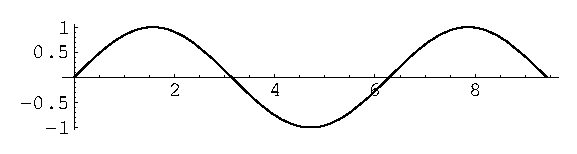
\includegraphics[width=8.5cm]{image1}}
%  \vspace{2.0cm}
  \centerline{(a) Result 1}\medskip
\end{minipage}
%
\begin{minipage}[b]{.48\linewidth}
  \centering
  \centerline{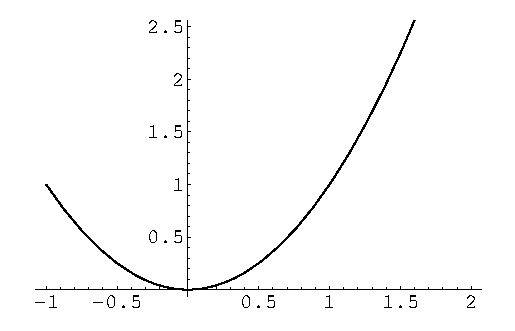
\includegraphics[width=4.0cm]{image3}}
%  \vspace{1.5cm}
  \centerline{(b) Results 3}\medskip
\end{minipage}
\hfill
\begin{minipage}[b]{0.48\linewidth}
  \centering
  \centerline{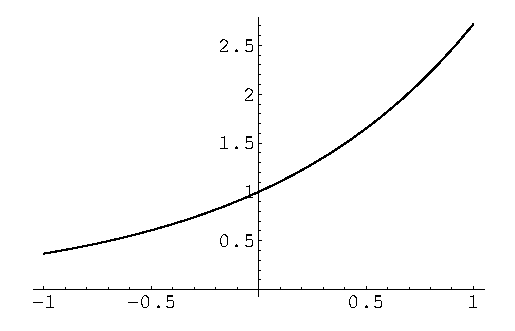
\includegraphics[width=4.0cm]{image4}}
%  \vspace{1.5cm}
  \centerline{(c) Result 4}\medskip
\end{minipage}
%
\caption{Example of placing a figure with experimental results.}
\label{fig:res}
%
\end{figure}


% To start a new column (but not a new page) and help balance the last-page
% column length use \vfill\pagebreak.
% -------------------------------------------------------------------------
%\vfill
%\pagebreak

\section{COPYRIGHT FORMS}
\label{sec:copyright}

You must include your fully completed, signed IEEE copyright release form when
form when you submit your paper. We {\bf must} have this form before your paper
can be published in the proceedings.

\section{REFERENCES}
\label{sec:ref}

List and number all bibliographical references at the end of the
paper. The references can be numbered in alphabetic order or in
order of appearance in the document. When referring to them in
the text, type the corresponding reference number in square
brackets as shown at the end of this sentence \cite{C2}. An
additional final page (the fifth page, in most cases) is
allowed, but must contain only references to the prior
literature.

% References should be produced using the bibtex program from suitable
% BiBTeX files (here: strings, refs, manuals). The IEEEbib.bst bibliography
% style file from IEEE produces unsorted bibliography list.
% -------------------------------------------------------------------------
\bibliographystyle{IEEEbib}
\bibliography{strings,refs}

\end{document}
